\section{Using the Visualisers and Views}
If this is the first time you use the \cjdt, switch to the \caesarj ~perspective by selecting \markedtext{Window} $\rightarrow$ \markedtext{Open Perspective} $\rightarrow$ \markedtext{Other}. Pick \markedtext{CaesarJDT Perspective} (see figure \ref{fig:select_persp}) in the list.

\begin{figure*}[htbp]
	\centering
		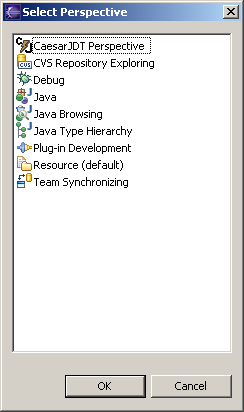
\includegraphics[width=0.35\textwidth]{images/select_persp.png}
	\caption{Perspective selection}
	\label{fig:select_persp}
\end{figure*}

This perspective extends the Java perspective. Especially a new view is available. The \markedtext{\caesarj ~Hierarchy View}. See section \ref{hierarchyview} for detailed information.\\
You can switch between the Java and Caesar Visualization perspectives using the perspective icons located in the top right of the menu bar.\\
\subsection{Outline view}
The outline view is showing structural members and crosscutting relationships. It extends the Java outline view by additional information (e.g advice declarations to the places it advises). A sample outline view bar is shown in figure \ref{fig:outline_view}.

\begin{figure*}[htbp]
	\centering
		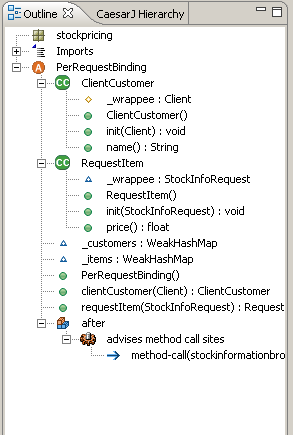
\includegraphics[width=0.35\textwidth]{images/outline.png}
	\caption{Outline View}
	\label{fig:outline_view}
\end{figure*}

\subsection{Hierarchy View\label{hierarchyview}}
% It displays the hierarchical relationships of \caesarj ~cclasses.
A \caesarj ~hierarchy view displays the hierarchical relationships of \caesarj ~cclasses. That means, that for each cclass their super-classes are displayed under the \markedtext{Super} node (see figure \ref{fig:hierarchy_view}). If the class contains nested classes (\markedtext{Contains} node) there are two displaying modes available for them:
\begin{itemize}
	\item[\textbf{Super:}] For each nested class their super classes are displayed.
	\item[\textbf{Sub:}] For each nested class their sub classes are displayed. If a sub class has two super classes the linearized inheritance relation is displayed in brackets after the class name.
\end{itemize}

\begin{figure*}[htbp]
	\centering
		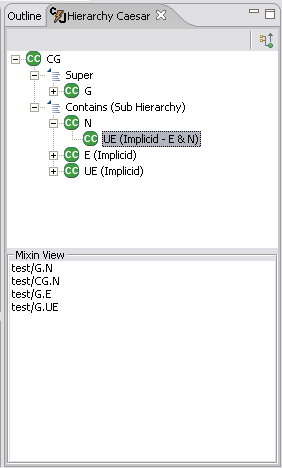
\includegraphics[width=0.35\textwidth]{images/hierarchy.png}
	\caption{\caesarj ~hierarchy view}
	\label{fig:hierarchy_view}
\end{figure*}

The modes can be switched by pressing the control button in the upper-right of the view. The second part of the view, named "Mixin view", shows the mixin composition of the currently selected (nested-) cclass.\\
\textbf{Note:} Since this view needs meta information from the compiler, the view refreshes when a project is (re-)built successfully.

\section{Common Problems and Limitations}
The \cjdt ~is under development. That is why there are some restrictions in this release. Some of these are listed below:
\begin{itemize}
	\item This release does not support live annotation while typing. To get this available, an \caesarj ~AST\footnote{Abstract Syntax Tree} would have to be built while changing code. This is not done yet.
	\item Showing the class hierarchy of an cclass marked in the editor by pressing \markedtext{F4}. Only the hierarchy view of an entire file and its included classes is supported.
	\item In-time refreshing of the outline bar and of the hierarchy view is not supported yet. In this release both of the views need meta information from the compiler. That is why they only refresh after a (re-) build of the entire project.
	\item It is not possible to declare breakpoints in cclasses, when debugging an \caesarj ~application.
\end{itemize}
